% Provenance (never printed): see sources/outline_sources.md (Year 2: natural hazards and risks
% quantified --- recurrence, probabilistic hazard, slope stability, tsunamis, floods, warning).
% Terminology from the UN report A/71/644 (UNDRR); the 475-year convention from the USGS
% Earthquake Hazards 201 page; the ground-motion prediction equation of Boore, Joyner and Fumal
% (USGS Open-File Report 93-509); run-ups from the NOAA NCEI tsunami database; the 1999 Vargas
% debris flows from USGS Open-File Report 01-0144. Ledger rows in sources/ledger/book4.md;
% curves and numbers from figdata/bachelor-2/hazards.py and the Book 4 second-writer scratch
% calculator calc/ch28.py. Hazards are described and quantified physically only: no advice.
\chapter{الأخطار الجيولوجية ومخاطرها}\label{ch:b2:geological-hazards}

إنّ مبنًى صُمِّم لتحمّل حركة الأرض التي تُتجاوز، في المتوسط، مرّة كلّ 475 سنة أمامه
فرصة واحدة من عشر لملاقاتها خلال عمر يبلغ خمسين سنة. والعبارتان رقم واحد
يُقرأ بطريقتين، والانتقال بينهما هو العمل اليومي لعلم الأخطار. ويبني هذا الفصل
أدواته: احتمال الأحداث النادرة، \omterm{def:b2:geological-hazards:psha}{ومنحنى الخطر} لموقع ما، واستقرار
المنحدر، وسرعة التسونامي وارتفاع صعوده، وتكرار الفيضانات، والفيزياء التي تحدّد
مقدار الإنذار الذي يمكن أن يتيحه كلّ خطر.
% ledger: usgs:eh201-475

\begin{recall}
\textbf{من مجلّدات المدرسة}: الخطر الطبيعي، والكارثة الطبيعية والانزلاق الأرضي؛ والهشاشة،
والمخاطر، والوقاية وخريطة الأخطار؛ والتسونامي؛ \omterm{def:b2:geological-hazards:return}{وفترة العودة} للفيضان، وصيغة الرتبة
$T = (n + 1)/m$ لسجلّ من $n$ من الذرى السنوية. \textbf{من مجلّد السنة الأولى}: قانون
غوتنبرغ--ريختر $\log_{10} N(\geq M) = a - bM$ وقيمة b فيه؛ والعزم الزلزالي وقدر
العزم؛ وضغط سائل المسام، والإجهاد الفعّال $\sigma' = \sigma - u$ ومعيار كولوم
للانهيار $\tau = c' + \sigma' \tan\varphi'$. \textbf{من \cref{ch:b2:eruptive-styles}}: التيارات الفتاتية
البركانية الكثيفة، \omterm{def:b2:eruptive-styles:lahar}{واللاهارات} وتساقط \omterm{def:b2:eruptive-styles:tephra}{التيفرا}. \textbf{من كتب الرياضيات}: توزيع بواسون
والتوزيع الأسّي، والتوزيع الطبيعي ودالّة توزيعه $\Phi$.
\textbf{من مجلّد السنة الثانية في كتب الفيزياء}: علاقة التشتّت لموجات الجاذبية السطحية،
$\omega^2 = gk\tanh(kh)$.
\end{recall}

\section{الخطر والتعرّض والمخاطر}\label{sec:b2:geological-hazards:risk}

\begin{definition}[الخطر الجيولوجي، التعرّض، مخاطر الكوارث]\label{def:b2:geological-hazards:risk}
\emph{الخطر الجيولوجي}\index{الخطر الجيولوجي} عملية أو ظاهرة تنشأ في
العمليات الداخلية للأرض --- زلزال، أو ثوران، أو حركة كتلية مثل
انزلاق أرضي أو \omterm{def:b2:geological-hazards:slope}{تدفّق حطام} --- وقد تسبّب خسائر في الأرواح، أو إصابات، أو أضرارًا أو اضطرابًا. ويتّسم
بموقعه، وشدّته أو قدره، وتكراره أو احتماله. و\emph{التعرّض}\index{التعرّض (لخطر)} لخطر ما
هو وضع الناس، والمباني، والبنى التحتية وسائر الأصول الواقعة حيث يمكن أن يبلغها الخطر،
ويقاس بعددها أو بقيمتها. و\emph{مخاطر الكوارث}\index{مخاطر الكوارث} هي الخسارة المحتملة
في الأرواح، أو الصحّة أو الأصول التي قد تقع في فترة معيّنة، وتُحدَّد احتماليًا
انطلاقًا من الخطر، والتعرّض وهشاشة ما هو معرَّض له.
\end{definition}
% ledger: undrr:hazard, undrr:geological, undrr:exposure, undrr:disaster-risk, undrr:vulnerability

وتصنّف المصطلحات الدولية التسونامي على حدة: فهو ينطلق بالزلازل وبأحداث
جيولوجية أخرى، ثم يصبح عملية محيطية ويضرب بوصفه خطرًا ساحليًا مرتبطًا بالماء.
ويعالجه هذا الفصل مع الأخطار الأخرى، لأنّ مصدره جيولوجي.
% ledger: undrr:geological

ويتضمّن التعريف جداءً. فإذا وقعت أحداث شدّتها $i$ بمعدّل سنوي
$\lambda_i$، وكانت قيمة الأصول المعرَّضة $E$، وكان الحدث ذو الشدّة $i$ يدمّر
كسرًا $V_i$ منها (الهشاشة، بين 0 و1)، فإنّ الخسارة السنوية المتوقّعة هي
\begin{equation}
L = \sum_i \lambda_i \, E \, V_i ,
\label{eq:b2:geological-hazards:loss}
\end{equation}
وكثيرًا ما تُختصر في: المخاطر = الخطر $\times$ \omterm{def:b2:geological-hazards:risk}{التعرّض} $\times$ الهشاشة. وتنعدم المخاطر حين
ينعدم أيّ عامل: بركان عنيف في جزيرة خالية، أو مدينة مزدحمة على كراتون هادئ، أو
مبانٍ تقاوم الاهتزاز. ويقيس علم الأخطار العامل الأول؛ ويضعه الشكل أدناه
بين العوامل الثلاثة.

\begin{omfigure}
\centering
\begin{tikzpicture}[font=\small]
\fill[omThm!14] (90:1.05) circle (1.55);
\fill[omDef!14] (210:1.05) circle (1.55);
\fill[black!8] (330:1.05) circle (1.55);
\begin{scope}
\clip (90:1.05) circle (1.55);
\clip (210:1.05) circle (1.55);
\fill[omThm!45!omDef!45] (330:1.05) circle (1.55);
\end{scope}
\draw[omThm, thick] (90:1.05) circle (1.55);
\draw[omDef, thick] (210:1.05) circle (1.55);
\draw[black!60, thick] (330:1.05) circle (1.55);
\node[align=center, anchor=south] at (0,2.65) {\foreignlanguage{arabic}{\textbf{الخطر} {\scriptsize (المعدّل $\lambda_i$، الشدّة)}}};
\node[align=right, anchor=east] at (-2.55,-1.35) {\foreignlanguage{arabic}{\textbf{التعرّض}}\\[-1pt]{\scriptsize\foreignlanguage{arabic}{الأصول $E$}}};
\node[align=left, anchor=west] at (2.55,-1.35) {\foreignlanguage{arabic}{\textbf{الهشاشة}}\\[-1pt]{\scriptsize\foreignlanguage{arabic}{الكسر المفقود $V_i$}}};
\node[align=center, font=\scriptsize\bfseries] at (0,0) {المخاطر};
\end{tikzpicture}
\par\smallskip{\small العوامل الثلاثة \omterm{def:b2:geological-hazards:risk}{لمخاطر الكوارث}. ولا تكون الخسارة المتوقّعة غير معدومة إلا حيث
تتداخل العوامل الثلاثة كلّها: خطر يبلغ شيئًا معرَّضًا له وقابلًا للتضرّر.}
\end{omfigure}

\section{احتمال الأحداث النادرة}\label{sec:b2:geological-hazards:probability}

\begin{definition}[فترة العودة]\label{def:b2:geological-hazards:return}
لنفترض أنّ أحداثًا من نوع معيّن --- فيضانًا يفوق تصريفًا ما، أو حركة أرضية تفوق مستوى ما، أو
زلزالًا يفوق قدرًا ما --- تقع بمعدّل سنوي متوسّط $\lambda$. إنّ \emph{فترة
العودة}\index{فترة العودة} لهذه الأحداث هي $T = 1/\lambda$: متوسّط الفاصل بين حدثين منها، ومقلوب
معدّلها السنوي، لا جدولًا زمنيًا.
\end{definition}
% ledger: usgs:eh201-475

\begin{definition}[احتمال التجاوز]\label{def:b2:geological-hazards:poisson}
\emph{احتمال التجاوز}\index{احتمال التجاوز} لمستوى ما خلال زمن تعرّض $t$
هو احتمال أن يُبلَغ المستوى أو يُتجاوز مرّة واحدة على الأقلّ خلال $t$.
\end{definition}

\begin{proposition}[نموذج بواسون للتكرار]\label{prop:b2:geological-hazards:poisson}
لنفترض أنّ الأحداث تقع واحدًا تلو الآخر\index{نموذج بواسون للتكرار}، مستقلّة بعضها عن
بعض وعن الزمن المنقضي، بمعدّل متوسّط ثابت $\lambda = 1/T$. عندئذ يتبع العدد $N$ من
الأحداث خلال زمن $t$ توزيعَ بواسون الذي متوسّطه $\lambda t$؛ ويكون \omterm{def:b2:geological-hazards:poisson}{احتمال
التجاوز} خلال $t$
\begin{equation}
P(t) = 1 - e^{-t/T};
\label{eq:b2:geological-hazards:poisson}
\end{equation}
ويتبع الفاصل بين حدثين متتاليين التوزيعَ الأسّي الذي متوسّطه $T$.
\end{proposition}

\begin{proof}
ليكن $P_k(t)$ احتمال وقوع $k$ حدثًا في $[0, t]$. في فاصل قصير $\mathrm{d}t$ يقع
حدث باحتمال $\lambda\,\mathrm{d}t$، بمعزل عن الماضي، ويقع حدثان باحتمال
من رتبة أعلى. ومن ثمّ $P_0(t + \mathrm{d}t) = P_0(t)(1 - \lambda\,\mathrm{d}t)$، أي
$P_0' = -\lambda P_0$ مع $P_0(0) = 1$: $P_0(t) = e^{-\lambda t}$، و$P(t) = 1 - P_0(t)$. وبالطريقة
نفسها $P_k' = \lambda(P_{k-1} - P_k)$ عندما $k \geq 1$، وتُحلّ بالاستقراء:
$P_k(t) = (\lambda t)^k e^{-\lambda t}/k!$، أي توزيع بواسون الذي متوسّطه $\lambda t$. وإذا انطلقنا من
حدث، أعطت الحجّة نفسها احتمال أن يأتي الحدث التالي بعد $t$:
$e^{-\lambda t}$، وهي دالّة البقاء للتوزيع الأسّي، الذي متوسّطه
$\int_0^\infty e^{-\lambda t}\,\mathrm{d}t = 1/\lambda = T$.
\end{proof}

وتُستعمل نتيجتان في كلّ مكان. فلاحتمال $p$ خلال زمن تعرّض $t$، تكون \omterm{def:b2:geological-hazards:return}{فترة
العودة} $T = -t/\ln(1 - p)$: فاحتمال \qty{10}{\percent} خلال 50 سنة يعطي $T = 50/0.10536 =
474.6$ سنة، وهي حركة «475 سنة» في قوانين البناء، واحتمال \qty{2}{\percent} خلال 50 سنة
يعطي 2475 سنة. وحين يكون $t \ll T$، يكون $P \approx t/T$: فيمكن قراءة المعدّل
احتمالًا في السنة. أمّا على مدى فترة عودة كاملة، فالاحتمال $1 - e^{-1} =
\qty{63}{\percent}$، لا 1. ويرسم الشكل أدناه (يمينًا) \eqref{eq:b2:geological-hazards:poisson}
لثلاث فترات عودة.
% ledger: usgs:eh201-475
% values: T 474.561 and 2474.92 years; P(50|475) 0.0999 (hazards.py numbers)

هل النموذج صحيح؟ يضمّ الفهرس العالمي للزلازل التي لا يقلّ قدرها عن 7 نحو 696 حدثًا
من 1976 إلى 2025، أي 695 فاصلًا متوسّطها 26.2 يومًا. ولو كانت عملية بواسون،
لكان كسر الفواصل الأطول من $t$ هو $e^{-t/26.2}$، أي خطًّا مستقيمًا على محور
لوغاريتمي. ويُظهر الشكل أدناه (يسارًا) أنّه يكاد يكون كذلك: فنسبة \qty{30.4}{\percent} من الفواصل
أطول من 30 يومًا، مقابل \qty{31.8}{\percent} وفق النموذج، والانحراف المعياري
للفواصل يساوي 1.07 مرّة متوسّطها، مقابل 1 تمامًا. والخلل في الفواصل القصيرة: إذ يقع 36 زوجًا
في اليوم نفسه، وهي هزّات لاحقة وأزواج زلزالية ما كانت عملية عديمة الذاكرة لتجمعها. ولذلك
تزيل خرائط الأخطار الأحداث التابعة من الفهرس، أي تفكّ تجمّعه، كي يمكن
معاملة الهزّات الرئيسية المتبقّية بوصفها عملية بواسون؛ وتأتي معدّلاتها بحسب القدر من
قانون غوتنبرغ--ريختر.
% ledger: data:usgs-comcat, usgs:eh201-poisson
% values: m7_events 696, mean 26.2245 d, cv 1.06891, same-day 36, frac>30 d 0.303597 vs 0.318552

\begin{omfigure}
\centering
\begin{minipage}[b]{0.49\linewidth}\centering
\begin{tikzpicture}
\begin{axis}[omrecord, width=0.96\linewidth, height=5.2cm, xmin=0, xmax=200, ymin=0, ymax=1,
  xlabel={زمن التعرّض $t$ (بالسنوات)}, ylabel={احتمال التجاوز},
  tick label style={font=\scriptsize}, label style={font=\small},
  xtick={0,50,100,150,200}, ytick={0,0.2,...,1}]
% computed in figdata/bachelor-2/hazards.py part poisson
\addplot[omThm, line width=1pt] table[x=t_yr, y=P50] {figdata/out/bachelor-2-hazards-poisson.dat};
\addplot[omDef, line width=1pt] table[x=t_yr, y=P475] {figdata/out/bachelor-2-hazards-poisson.dat};
\addplot[black!70, line width=1pt, densely dashed] table[x=t_yr, y=P2475] {figdata/out/bachelor-2-hazards-poisson.dat};
\draw[black!50, densely dotted] (axis cs:50,0) -- (axis cs:50,1);
\fill[omDef] (axis cs:50,0.1) circle (1.8pt);
\node[font=\scriptsize, text=omThm, anchor=west] at (axis cs:62,0.86) {$T = 50$};
\node[font=\scriptsize, text=omDef, anchor=west] at (axis cs:120,0.34) {$T = 475$};
\node[font=\scriptsize, text=black!70, anchor=west] at (axis cs:120,0.12) {$T = 2475$};
\node[font=\scriptsize, anchor=west, text=omDef] at (axis cs:52,0.2) {\qty{10}{\percent}};
\end{axis}
\end{tikzpicture}
\end{minipage}\hfill
\begin{minipage}[b]{0.49\linewidth}\centering
\begin{tikzpicture}
\begin{axis}[omrecord, width=0.93\linewidth, height=5.2cm, xmin=0, xmax=120, ymode=log,
  ymin=0.008, ymax=1.1, xlabel={الفاصل $t$ (بالأيام)}, ylabel={كسر الفواصل $> t$},
  tick label style={font=\scriptsize}, label style={font=\small}, xtick={0,30,60,90,120},
  legend style={at={(0.03,0.03)}, anchor=south west, font=\scriptsize, draw=black!30},
  legend cell align=left]
% computed in figdata/bachelor-2/hazards.py part survival; ledger: data:usgs-comcat
\addplot[omThm, only marks, mark=*, mark size=1.2pt] table[x=t_day, y=observed] {figdata/out/bachelor-2-hazards-survival.dat};
\addlegendentry{\foreignlanguage{arabic}{الزلازل $M \geq 7$ في الفترة 1976--2025}}
\addplot[black, line width=0.9pt] table[x=t_day, y=poisson] {figdata/out/bachelor-2-hazards-survival.dat};
\addlegendentry{\foreignlanguage{arabic}{بواسون، بمتوسّط 26.2 يومًا}}
\end{axis}
\end{tikzpicture}
\end{minipage}
\par\smallskip{\small يمينًا: احتمال وقوع حدث واحد على الأقلّ خلال زمن تعرّض $t$ في
فترات عودة تبلغ 50 و475 و2475 سنة؛ وللحدث ذي \omterm{def:b2:geological-hazards:return}{فترة العودة} 475 سنة فرصة \qty{10}{\percent} خلال 50
سنة. يسارًا: الفواصل بين الزلازل البالغ عددها 696 التي لا يقلّ قدرها عن 7 في الفهرس
العالمي للفترة 1976--2025، مقابل القانون الأسّي لعملية بواسون لها المعدّل نفسه. البيانات:
الفهرس الشامل لشبكة ANSS التابعة لهيئة المسح الجيولوجي الأمريكية (USGS).}
\end{omfigure}

\section{الخطر الزلزالي}\label{sec:b2:geological-hazards:seismic}

\begin{definition}[التحليل الاحتمالي للخطر الزلزالي، معادلة التنبّؤ بحركة الأرض، أقصى تسارع للأرض، منحنى الخطر]\label{def:b2:geological-hazards:psha}
\emph{أقصى تسارع للأرض}\index{أقصى تسارع للأرض} (PGA) في موقع ما هو أكبر
تسارع أفقي مطلق للأرض خلال زلزال، ويُعبَّر عنه عادة
كسرًا من $g$. و\emph{معادلة التنبّؤ بحركة الأرض}\index{معادلة التنبّؤ بحركة الأرض}
(GMPE) تعطي التوزيع الاحتمالي لمقياس للاهتزاز، مثل أقصى التسارع، في
موقع ما --- وسيطًا وتشتّتًا --- بدلالة القدر، والمسافة إلى المصدر
وأحوال الأرض. و\emph{التحليل الاحتمالي للخطر الزلزالي}\index{التحليل الاحتمالي للخطر الزلزالي}
(PSHA) يجمع كلّ الزلازل التي يمكن أن تؤثّر في موقع ما، بمعدّلاتها ومسافاتها،
مع معادلة للتنبّؤ بحركة الأرض، ليعطي المعدّل السنوي الذي يُتجاوز به كلّ مستوى من الاهتزاز.
ومنحنى هذا المعدّل بدلالة المستوى هو \emph{منحنى
الخطر}\index{منحنى الخطر} للموقع.
\end{definition}
% ledger: usgs:eh201-pga, usgs:eh201-475

إنّ أقصى التسارع هو ما تتعرّض له جسيمة من الأرض. أمّا المبنى فيستجيب لجزء الحركة
القريب من دوره الطبيعي، وترسم قوانين البناء خرائط لتلك الاستجابة أيضًا، أي التسارع الطيفي؛
ويُبقي أقصى التسارع الاستدلالَ بسيطًا، ولذا يُستعمل هنا.
% ledger: usgs:eh201-pga

\begin{method}[تحليل احتمالي للخطر الزلزالي]\label{met:b2:geological-hazards:psha}
\begin{enumerate}
  \item \textbf{المصادر.} ارسم خرائط للصدوع ومناطق المصادر حول الموقع، وللمسافة $d$ بين
        كلّ منها والموقع.
  \item \textbf{التكرار.} لكلّ مصدر، خذ المعدّل السنوي للزلازل بحسب القدر
        من قانون غوتنبرغ--ريختر مبتور عند قدر أقصى $M_{\max}$:
        $N(\geq m) = 10^{a - bm} - 10^{a - bM_{\max}}$، بدءًا من قدر أدنى $M_{\min}$.
        وقسّم المدى إلى شرائح معدّلها $\nu_j$ حول الأقدار $m_j$.
  \item \textbf{حركة الأرض.} من \omterm{def:b2:geological-hazards:psha}{معادلة التنبّؤ بحركة الأرض}، خذ الوسيط $\mu_j = \log_{10}\mathrm{PGA}$
        والتشتّت $\sigma$ لكلّ شريحة؛ ويكون احتمال أن يتجاوز أقصى التسارع القيمة $a$ هو
        $1 - \Phi\bigl((\log_{10} a - \mu_j)/\sigma\bigr)$.
  \item \textbf{الجمع.} المعدّل السنوي لتجاوز $a$ هو $\lambda(a) = \sum_j \nu_j
        \bigl[1 - \Phi\bigl((\log_{10} a - \mu_j)/\sigma\bigr)\bigr]$، مجموعًا على كلّ المصادر.
  \item \textbf{القراءة.} إنّ أقصى التسارع ذا الاحتمال $p$ للتجاوز خلال $t$ سنة هو المستوى الذي
        يكون عنده $\lambda(a) = -\ln(1 - p)/t$: أي \num{2.107e-3} في السنة لاحتمال \qty{10}{\percent} خلال 50 سنة.
\end{enumerate}
\end{method}

\omterm{def:b2:geological-hazards:psha}{ومعادلة التنبّؤ بحركة الأرض} المستعملة في هذا الفصل هي معادلة بور وجوينر وفومال، المعايَرة على 271 تسجيلًا
لعشرين زلزالًا في غرب أمريكا الشمالية: للمركّبة الأفقية العشوائية، بوحدات $g$،
\begin{equation}
\log_{10}\mathrm{PGA} = -0.105 + 0.229\,(M - 6) - 0.778\log_{10} r + 0.162\,G_B + 0.251\,G_C,
\qquad r = \sqrt{d^2 + 5.57^2},
\label{eq:b2:geological-hazards:gmpe}
\end{equation}
حيث $M$ قدر العزم، و$d$ المسافة بالكيلومترات إلى الإسقاط السطحي
للتمزّق، والتشتّت $\sigma = 0.230$ حول الوسيط. وهي صالحة عندما $5.0 \leq M \leq 7.7$ و$d
\leq \qty{100}{km}$. والثابت \qty{5.57}{km} عمق وهمي عايرَه الانحدار،
ويُبقي الحركة محدودة فوق المصدر. فزلزال قدره 6 على بعد \qty{15}{km} يعطي وسيطًا قدره
\qty{0.091}{g}، وزلزال قدره 7.5 يعطي \qty{0.200}{g}؛ والانحراف المعياري الواحد يضرب
الوسيط في $10^{0.230} = 1.70$ أو يقسمه عليه.
% ledger: bjf93:pga, bjf97:pga-ln
% values: M6@15 km 0.0908 g, M7.5@15 km 0.2003 g (hazards.py numbers)

ويحمل الحدّان $G_B$ و$G_C$ أثر الموقع. وتُصنَّف المواقع بحسب متوسّط سرعة موجات القصّ
في الطبقة العليا منها البالغ سمكها \qty{30}{m}: الصنف A فوق \qty{750}{m.s^{-1}} ($G_B = G_C = 0$)، والصنف B من
360 إلى \qty{750}{m.s^{-1}} ($G_B = 1$) والصنف C من 180 إلى \qty{360}{m.s^{-1}} ($G_C = 1$). والأرض
الليّنة تضرب حركة الصخر في $10^{0.162} = 1.45$ في الصنف B وفي $10^{0.251} = 1.78$ في الصنف
C: فالموجة التي تدخل مادّة أبطأ تتباطأ، ويقصر طولها وتكبر سعتها، ويمكن لطبقة ليّنة أو
لحوض مملوء بالرواسب أن يرنّ ويحبسها.
% ledger: bjf93:pga

ويطبّق الشكل أدناه الطريقة على منطقة مصدر واحدة تبعد \qty{15}{km} عن موقع صخري، مع $a
= 4.0$، و$b = 1.0$، و$M_{\min} = 5$ و$M_{\max} = 7.5$: أي نحو 0.1 زلزال قدره 5 أو
أكثر في السنة. وعند قيم أقصى التسارع الصغيرة يؤول المنحنى إلى هذا المعدّل، لأنّ كلّ زلزال يتجاوز
مستوى ضعيفًا. وأقصى التسارع ذو احتمال \qty{10}{\percent} خلال 50 سنة هو \qty{0.22}{g}. ولو أنّ كلّ زلزال أحدث
وسيطه تمامًا، لبُلغ المعدّل نفسه عند \qty{0.13}{g}، ولما أمكن أبدًا تجاوز أيّ مستوى أعلى من وسيط
أكبر زلزال، أي \qty{0.20}{g}. والتشتّت هو الذي يهيمن على المستويات
النادرة: فحركة \omterm{def:b2:geological-hazards:return}{فترة العودة} 475 سنة تأتي في معظمها من زلازل متوسّطة تهزّ أقوى من
وسيطها.
% values: psha_rate_m5 0.0997, psha_pga475 0.220894, psha_pga475_median 0.125607, median M7.5 0.2003 (hazards.py numbers)

\begin{omfigure}
\centering
\begin{tikzpicture}
\begin{axis}[omrecord, width=0.8\linewidth, height=5.6cm, xmode=log, ymode=log, xmin=0.01,
  xmax=2, ymin=1e-6, ymax=0.3, xlabel={أقصى تسارع للأرض \babelsublr{(\unit{g})}},
  ylabel={المعدّل السنوي للتجاوز}, unbounded coords=jump,
  tick label style={font=\scriptsize}, label style={font=\small},
  xtick={0.01,0.03,0.1,0.3,1}, xticklabels={0.01,0.03,0.1,0.3,1},
  legend style={at={(0.03,0.03)}, anchor=south west, font=\scriptsize, draw=black!30},
  legend cell align=left]
% computed in figdata/bachelor-2/hazards.py part psha; ledger: bjf93:pga
\addplot[omThm, line width=1.2pt] table[x=pga_g, y=rate] {figdata/out/bachelor-2-hazards-psha.dat};
\addlegendentry{مع تشتّت معادلة التنبّؤ}
\addplot[black!60, line width=1pt, densely dashed] table[x=pga_g, y=rate_median] {figdata/out/bachelor-2-hazards-psha.dat};
\addlegendentry{الأوساط وحدها}
\draw[omDef, densely dotted, thick] (axis cs:0.01,2.107e-3) -- (axis cs:2,2.107e-3);
\draw[omDef, densely dotted, thick] (axis cs:0.2209,1e-6) -- (axis cs:0.2209,2.107e-3);
\node[font=\scriptsize, text=omDef, anchor=south east] at (axis cs:2,2.107e-3) {\foreignlanguage{arabic}{احتمال \qty{10}{\percent} خلال 50 سنة}};
\node[font=\scriptsize, text=omDef, anchor=west] at (axis cs:0.235,2e-5) {\qty{0.22}{g}};
\end{axis}
\end{tikzpicture}
\par\smallskip{\small منحنى خطر: المعدّل السنوي الذي يتجاوز به أقصى تسارع الأرض في موقع صخري كلّ
مستوى، لمنطقة مصدر واحدة على بعد \qty{15}{km} (تكرار غوتنبرغ--ريختر مبتور، $b = 1$،
وأقدار من 5 إلى 7.5) ومعادلة التنبّؤ لبور وجوينر وفومال. وتقرأ الخطوط المنقّطة
مستوى احتمال \qty{10}{\percent} خلال 50 سنة. ومن دون التشتّت (المتقطّع) يتوقّف المنحنى عند وسيط
حركة أكبر زلزال.}
\end{omfigure}

\section{الخطر البركاني}\label{sec:b2:geological-hazards:volcanic}

يهدّد البركان عبر عدّة عمليات في آن واحد، لكلّ منها مداها: \omterm{def:b2:eruptive-styles:tephra}{فالتيفرا} تتساقط بعيدًا
مع اتجاه الريح، والتيارات الفتاتية البركانية الكثيفة \omterm{def:b2:eruptive-styles:lahar}{واللاهارات} تتبع الأودية، وتتقدّم تدفّقات الحمم ببطء
(\cref{ch:b2:eruptive-styles}). وترسم خريطة أخطاره منطقة لكلّ منها، انطلاقًا من رواسب الثورانات
السابقة ومن نماذج للتدفّق والتساقط. وتُبنى الاحتمالات بطريقة تختلف عن احتمالات
الزلازل، لأنّ البركان الذي يستيقظ ليس عملية مستقرّة. وتقود شجرة الأحداث
من الاضطراب إلى النتائج عبر فروع، كلّ منها من حدث سابق ضروري إلى نتيجة
أكثر تحديدًا --- اضطراب صهاري أو غير صهاري؛ ثوران أو لا؛ انفجاري أو انسيابي؛ تدفّق فتاتي بركاني
يبلغ واديًا معيّنًا أو لا. واحتمال نتيجة ما هو جداء الاحتمالات الشرطية
على طول فرعها. فإذا كان $M$ اضطرابًا صهاريًا، و$E$ ثورانًا، و$X$ \omterm{def:b2:eruptive-styles:regimes}{ثورانًا
انفجاريًا} و$V$ تدفّقًا في الوادي، فإنّ
\begin{equation*}
P(V) = P(M) \, P(E \mid M) \, P(X \mid E) \, P(V \mid X),
\end{equation*}
حيث يُقدَّر كلّ عامل من ماضي البركان، أو من براكين مماثلة أو من نماذج، ويُراجَع
بمبرهنة بايز كلّما وصلت بيانات رصد جديدة (\cref{exo:b2:geological-hazards:8}).
% ledger: nh02:event-tree

\section{الانزلاقات الأرضية}\label{sec:b2:geological-hazards:landslides}

يظلّ المنحدر قائمًا ما دامت مقاومة مادّته، على أيّ سطح يمكن أن ينزلق عليه،
تفوق الإجهاد الذي تطبّقه الجاذبية هناك. والمقاومة هي معيار كولوم في مجلّد السنة
الأولى، مكتوبًا بدلالة الإجهاد الفعّال: فالماء في المسام يحمل جزءًا من الحمل العمودي
ويخفّض الاحتكاك.

\begin{definition}[معامل الأمان، تدفّق الحطام]\label{def:b2:geological-hazards:slope}
\emph{معامل الأمان}\index{معامل الأمان} $F$ لمنحدر على طول سطح انزلاق محتمل
هو نسبة مقاومة القصّ المتاحة على السطح إلى إجهاد القصّ اللازم
للتوازن. ويكون المنحدر مستقرًّا عندما $F > 1$ وينهار حين ينخفض $F$ إلى 1. و\emph{تدفّق الحطام}\index{تدفّق الحطام}
جريان سريع لمزيج مشبع بالماء من الوحل، والرمل، والحصى، والجلاميد والخشب
يتحرّك نازلًا في قناة كتلةً واحدة كثيفة، تحمل الحبيبات جزءًا كبيرًا من وزنها، وينتشر
على المروحة عند مخرج القناة.
\end{definition}

\begin{proposition}[المنحدر اللانهائي]\label{prop:b2:geological-hazards:infinite-slope}
طبقة من التربة وزنها النوعي $\gamma$ وسمكها $z$، مقيسًا رأسيًا، ترتكز على سطح انزلاق
موازٍ للأرض بزاوية $\beta$؛ ومقاومتها $c'$ و$\varphi'$، وضغط
المسام على السطح $u = r_u \gamma z$. فإذا كانت الطبقة طويلة بما يكفي
لإهمال طرفيها، فإنّ
\begin{equation}
F = \frac{c' + \gamma z\,(\cos^2\beta - r_u)\tan\varphi'}{\gamma z \sin\beta\cos\beta}.
\label{eq:b2:geological-hazards:infinite-slope}
\end{equation}
لطبقة جافّة عديمة التماسك، $F = \tan\varphi'/\tan\beta$: فهي تظلّ قائمة حتى $\beta = \varphi'$.
\end{proposition}

\begin{proof}
خذ عمودًا من الطبقة عرضه الأفقي $b$. وزنه $W = \gamma z b$ لكلّ وحدة طول
عبر المنحدر، وقاعدته، الموازية للسطح، طولها $b/\cos\beta$. والقوى المؤثّرة في
جانبيه متساوية ومتعاكسة في منحدر لانهائي فتلغي إحداها الأخرى. وبتحليل $W$ عموديًا
وموازيًا للقاعدة، والقسمة على طولها، يكون الإجهادان العمودي والقصّي على القاعدة
$\sigma = \gamma z\cos^2\beta$ و$\tau = \gamma z \sin\beta\cos\beta$. والإجهاد العمودي الفعّال
هو $\sigma' = \sigma - u = \gamma z(\cos^2\beta - r_u)$، والمقاومة المتاحة $c' +
\sigma'\tan\varphi'$، و$F$ نسبتهما. ومع $c' = 0$ و$r_u = 0$، يكون $F = \cos^2\beta
\tan\varphi'/(\sin\beta\cos\beta) = \tan\varphi'/\tan\beta$.
\end{proof}

\begin{omfigure}
\centering
\begin{minipage}[b]{0.49\linewidth}\centering
\begin{tikzpicture}[scale=0.82, font=\scriptsize]
\def\t{0.57735}
\fill[black!10] (0,-1) -- (5.6,{5.6*\t-1}) -- (5.6,-1.6) -- (0,-1.6) -- cycle;
\fill[omThm!12] (0,0) -- (5.6,{5.6*\t}) -- (5.6,{5.6*\t-1}) -- (0,-1) -- cycle;
\draw[thick] (0,0) -- (5.6,{5.6*\t});
\draw[omDef, densely dashed] (0,-0.4) -- (5.6,{5.6*\t-0.4});
\draw[omThm, very thick] (0,-1) -- (5.6,{5.6*\t-1});
\fill[white, opacity=0.55] (2.4,{2.4*\t}) -- (3.2,{3.2*\t}) -- (3.2,{3.2*\t-1}) -- (2.4,{2.4*\t-1}) -- cycle;
\draw[black!75] (2.4,{2.4*\t}) -- (3.2,{3.2*\t}) -- (3.2,{3.2*\t-1}) -- (2.4,{2.4*\t-1}) -- cycle;
\draw[->, thick] (2.8,{2.8*\t-0.3}) -- (2.8,{2.8*\t-1.35}) node[below] {$W$};
\draw[<->] (4.6,{4.6*\t-1}) -- (4.6,{4.6*\t}) node[midway, right] {$z$};
\draw[black!60] (0.25,-1) -- (1.45,-1);
\draw[black!60] (1.25,-1) arc (0:30:1.0);
\node at (1.55,-0.78) {$\beta$};
\node[omDef, anchor=north, rotate=30, inner sep=1.5pt] at (1.3,{1.3*\t-0.4}) {المنسوب المائي};
\node[omThm, anchor=north, rotate=30] at (4.4,{4.4*\t-1.05}) {سطح الانزلاق};
\end{tikzpicture}
\end{minipage}\hfill
\begin{minipage}[b]{0.49\linewidth}\centering
\begin{tikzpicture}
\begin{axis}[omrecord, width=0.97\linewidth, height=5.2cm, xmin=0, xmax=0.5, ymin=0.5, ymax=2,
  xlabel={نسبة ضغط المسام $r_u$}, ylabel={معامل الأمان $F$},
  tick label style={font=\scriptsize}, label style={font=\small}, xtick={0,0.1,...,0.5},
  /pgf/number format/fixed]
% computed in figdata/bachelor-2/hazards.py part slope
\addplot[omDef, line width=1pt] table[x=r_u, y=F25] {figdata/out/bachelor-2-hazards-slope.dat};
\addplot[black, line width=1pt] table[x=r_u, y=F30] {figdata/out/bachelor-2-hazards-slope.dat};
\addplot[omThm, line width=1pt] table[x=r_u, y=F35] {figdata/out/bachelor-2-hazards-slope.dat};
\draw[black!50, densely dashed] (axis cs:0,1) -- (axis cs:0.5,1);
\node[font=\scriptsize, text=omDef, anchor=south west] at (axis cs:0.02,1.80) {\ang{25}};
\node[font=\scriptsize, anchor=south west] at (axis cs:0.02,1.50) {\ang{30}};
\node[font=\scriptsize, text=omThm, anchor=north west] at (axis cs:0.01,1.19) {\ang{35}};
\node[font=\scriptsize, text=black!60, anchor=north east] at (axis cs:0.5,0.98) {انهيار};
\end{axis}
\end{tikzpicture}
\end{minipage}
\par\smallskip{\small يمينًا: المنحدر اللانهائي، طبقة سمكها $z$ على سطح انزلاق موازٍ
للأرض، مع عمود وزنه $W$. يسارًا: \omterm{def:b2:geological-hazards:slope}{معامل أمانه} بدلالة نسبة ضغط
المسام، عندما $c' = \qty{5}{kPa}$، و$\varphi' = \ang{35}$، و$\gamma = \qty{19}{kN.m^{-3}}$ و$z =
\qty{2}{m}$، لثلاث زوايا ميل. وارتفاع ضغط المسام يقود كلّ منحدر إلى الانهيار.}
\end{omfigure}
% values: F(r_u = 0) 1.845, 1.517, 1.280; r_u at F = 1: 0.462, 0.320, 0.188 (calc/ch28.py)

تسمّي المعادلة \eqref{eq:b2:geological-hazards:infinite-slope} المحفّزين الشائعين. فالمطر
يرفع منسوب المياه الجوفية ومعه $r_u$؛ وينخفض $F$ خطّيًا مع $r_u$، بحيث إنّ منحدرًا
آمنًا وهو جافّ ينهار وهو رطب: ففي الشكل أعلاه، ينهار المنحدر ذو الزاوية \ang{35} عند $r_u = 0.19$، والمنحدر ذو
الزاوية \ang{25} لا ينهار إلا عند 0.46. ويضيف الاهتزاز قوّة أفقية: فإذا مُثّلت بالقوّة $kW$، حيث $k$
كسر من $g$، فقد البسط المقدار $\gamma z k \sin\beta\cos\beta\tan\varphi'$ وكسب
المقام $\gamma z k\cos^2\beta$ --- وهو تحليل شبه سكوني، مُسلَّم به هنا، يستبدل
باهتزاز قصير قوّةً ثابتة. وحدّ التماسك، $c'/(\gamma z\sin\beta\cos\beta)$،
يتناقص كلّما ازداد سمك الطبقة، فالتماسك يحمي الترب الرقيقة أكثر من العميقة.

في ديسمبر 1999 أسقطت عاصفة دامت ثلاثة أيام \qty{911}{mm} من المطر على مايكيتيا، على الساحل
شمال كاراكاس. وانطلقت آلاف الانزلاقات الأرضية الضحلة على منحدرات سييرا دي أفيلا،
على منحدرات من \ang{30} إلى أكثر من \ang{60}، و\ang{42} في المتوسط. وفي القنوات اندمجت
في \omterm{def:b2:geological-hazards:slope}{تدفّقات حطام}، تحرّكت بسرعات من 3 إلى \qty{14}{m.s^{-1}} قُدّرت من ارتفاع سطحها
في المنعطفات، وحملت جلاميد يبلغ طولها \qty{11}{m}. وعلى مروحة كارابايّيدا، المبيّنة أدناه،
تركت ما يصل إلى \qty{6}{m} من الحطام الجلمودي، أي نحو 1.8 مليون متر مكعب. ويُذكر عدد القتلى
عمومًا بنحو \num{30000}.
% ledger: vargas:storm, vargas:slopes, vargas:velocity, vargas:caraballeda, vargas:deaths

\begin{omfigure}
\centering
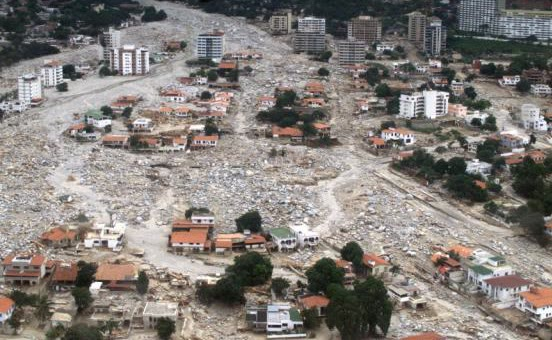
\includegraphics[width=0.62\linewidth]{images/book4/b2-28-caraballeda-debris-flow.jpg}
\par\smallskip{\small رواسب \omterm{def:b2:geological-hazards:slope}{تدفّقات الحطام} على مروحة كارابايّيدا، على ساحل فنزويلا،
بعد عاصفة ديسمبر 1999: فقد غادرت التدفّقات القناة الرئيسية ودفنت البلدة تحت
الجلاميد. الصورة: \mbox{\textdir TLT Lawson Smith}، فيلق المهندسين في الجيش الأمريكي (ملك عام).}
\end{omfigure}
% ledger: photo:b2-28-caraballeda, vargas:caraballeda

\section{التسونامي}\label{sec:b2:geological-hazards:tsunamis}

للتسونامي الذي يُحدثه ارتفاع مفاجئ لقاع البحر طول موجي يبلغ عشرات إلى مئات
الكيلومترات، أي أكبر بكثير من عمق المحيط. فهو موجة طويلة، وسرعته لا تتوقّف إلا
على العمق.

\begin{proposition}[الموجات الطويلة]\label{prop:b2:geological-hazards:long-waves}
موجة الجاذبية السطحية التي يفوق طولها الموجي عمق الماء $h$ بكثير تنتقل
بالسرعة $c = \sqrt{gh}$، أيًّا كان طولها الموجي. وحيث تتحرّك ببطء نحو مياه أضحل من دون
أن تنعكس أو تنكسر، تكبر سعتها $A$ بحسب $h^{-1/4}$.
\end{proposition}

\begin{proof}
تعطي علاقة التشتّت سرعة الطور $c = \omega/k = \sqrt{(g/k)\tanh(kh)}$. وللموجة
الطويلة $kh = 2\pi h/\lambda \ll 1$، و$\tanh(kh) \approx kh$، فيكون $c = \sqrt{gh}$، مستقلًّا عن
$k$: فالموجات الطويلة لا تتشتّت. وطاقة الموجة لكلّ وحدة مساحة من سطح البحر $\frac12
\rho g A^2$، وهي تنتقل بالسرعة $c$. فإذا لم ينعكس شيء من الطاقة ولم يُفقد، كان التدفّق $\frac12\rho g A^2
c$ عبر أيّ مقطع ثابتًا على طول المسار: فالمقدار $A^2 \sqrt{h}$ ثابت، و$A \propto
h^{-1/4}$.
\end{proof}

فوق \qty{4000}{m} من الماء ينتقل التسونامي بسرعة \qty{198}{m.s^{-1}}، أي \qty{713}{km/h}؛ وفوق
\qty{5000}{m}، بسرعة \qty{797}{km/h}، وهي عبارة «أكثر من 800 كيلومتر في الساعة» التي تذكرها خدمات الإنذار. وقرب
الشاطئ، في \qty{10}{m} من الماء، يتباطأ إلى \qty{36}{km/h}؛ فتلحق بمقدّمته المياه
التي خلفها، فتقصر الموجة ويشتدّ انحدارها، ويزداد ارتفاعها.
% ledger: nws:tsunami-speed

\begin{definition}[ارتفاع صعود التسونامي]\label{def:b2:geological-hazards:tsunami}
\emph{ارتفاع صعود التسونامي}\index{ارتفاع صعود التسونامي} عند نقطة من الساحل هو ارتفاع أعلى
أرض يبلغها الماء في الداخل هناك، فوق مستوى سطح البحر في ذلك الوقت. والمسافة الأفقية
من خطّ الشاطئ إلى تلك النقطة هي مسافة الغمر.
\end{definition}

تقيس فرق المسح ارتفاعات الصعود من علامات الماء، وخطوط الحطام والأضرار بعد كلّ تسونامي. وتضمّ
قاعدة بيانات التسونامي العالمية \num{2177} رصدًا لارتفاع الصعود لتسونامي المحيط الهندي في
26 ديسمبر 2004، الذي أحدثه زلزال قدره 9.1 قبالة سومطرة، بأقصى ارتفاع للماء بلغ
\qty{50.9}{m}، و\num{6429} رصدًا لتسونامي 11 مارس 2011 قبالة هونشو، وقدره 9.1 أيضًا،
بأقصى ارتفاع بلغ \qty{39.3}{m}. وقد أودى الأوّل بحياة \num{227899} شخصًا والثاني بحياة \num{18423}. وفي باندا آتشيه،
بلغ الماء منتصف الطابق الثاني من المسجد المبيّن أدناه.
% ledger: ncei:tsu-2004, ncei:tsu-2011, usgs:aceh-mosque

\begin{omfigure}
\centering
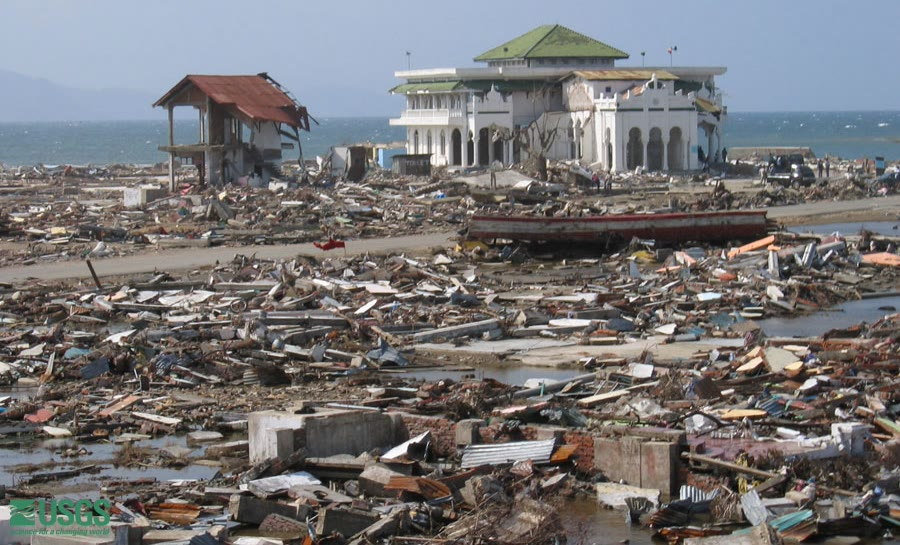
\includegraphics[width=0.62\linewidth]{images/book4/b2-28-aceh-mosque-tsunami.jpg}
\par\smallskip{\small باندا آتشيه، سومطرة، في 21 يناير 2005، بعد تسونامي 26 ديسمبر
2004: مسجد قائم وسط أنقاض المباني المحيطة به. الصورة: هيئة المسح
الجيولوجي الأمريكية (ملك عام).}
\end{omfigure}
% ledger: photo:b2-28-aceh

\section{الفيضانات}\label{sec:b2:geological-hazards:floods}

\begin{definition}[منحنى تكرار الفيضانات]\label{def:b2:geological-hazards:flood}
\emph{منحنى تكرار الفيضانات}\index{منحنى تكرار الفيضانات} لنهر عند محطّة قياس هو
منحنى ذروة التصريف السنوية بدلالة فترة عودتها، أو احتمال تجاوزها
السنوي، ويُبنى من سجلّ المحطّة للذرى السنوية ويُمدَّد عادة بقانون احتمالي
معايَر.
\end{definition}

وصيغة الرتبة في مجلّدات المدرسة هي التي تحدّد مواقع نقاط المنحنى. ولها مسوّغ.

\begin{proposition}[موقع الرسم لويبول]\label{prop:b2:geological-hazards:weibull}
لتكن $n$ ذروة سنوية مستقلّة ومسحوبة من التوزيع المتّصل نفسه، وليكن
$G(x)$ احتمال أن تتجاوز ذروة سنة ما القيمة $x$. فالذروة ذات الرتبة $m$، معدودةً من
الأكبر، لها احتمال تجاوز متوقّع $m/(n + 1)$، ولذا تُرسم عند $T = (n +
1)/m$.
\end{proposition}

\begin{proof}
المتغيّر $U = G(X)$ منتظم على $[0, 1]$ لقانون متّصل، و$G$ متناقصة، فتقابل
الذروة رقم $m$ من حيث الكبر القيمة رقم $m$ من حيث الصغر بين $n$ متغيّرات منتظمة مستقلّة،
$U_{(m)}$. وكثافتها $f(u) = \frac{n!}{(m-1)!\,(n-m)!}u^{m-1}(1-u)^{n-m}$: قيمة واحدة من القيم البالغ عددها $n$
عند $u$، و$m - 1$ تحتها و$n - m$ فوقها. ومع تكامل بيتا $\int_0^1 u^{p}(1-u)^{q}\,\mathrm{d}u
= p!\,q!/(p + q + 1)!$،
\begin{equation*}
\mathbb{E}[U_{(m)}] = \frac{n!}{(m-1)!\,(n-m)!}\cdot\frac{m!\,(n-m)!}{(n+1)!} = \frac{m}{n+1}. \qedhere
\end{equation*}
\end{proof}

فأكبر ذروة في سجلّ من 30 سنة تُرسم إذن عند 31 سنة، ولا شيء في السجلّ يحدّد
فيضان المئة سنة. وللوصول إليه، تُعايَر الذرى بقانون للقيم القصوى، وغالبًا ما يكون قانون غومبل،
$\Pr(\text{الذروة} \leq x) = \exp\bigl(-e^{-(x - u)/\alpha}\bigr)$، الذي يكون فيه فيضان $T$ سنة هو $x_T = u
- \alpha\ln\bigl(-\ln(1 - 1/T)\bigr)$: أي خطّ مستقيم بدلالة $-\ln(-\ln(1 - 1/T))$، يُستقرأ
خارج السجلّ بمجازفة تزداد مع البعد عنه.

\section{الرصد والإنذار المبكر}\label{sec:b2:geological-hazards:warning}

\begin{definition}[نظام الإنذار المبكر]\label{def:b2:geological-hazards:warning}
\emph{نظام الإنذار المبكر}\index{نظام الإنذار المبكر} نظام متكامل لرصد الخطر،
والتنبّؤ به، وتقييم المخاطر، والتواصل والتأهّب، يتيح التصرّف في الوقت المناسب
قبل وقوع حدث خطِر. ويجمع أربعة عناصر: معرفة المخاطر؛ وكشف الخطر،
ورصده والتنبّؤ به؛ ونشر الإنذارات؛ والتأهّب
للاستجابة.
\end{definition}
% ledger: undrr:ews

تحدّد الفيزياء مقدار الوقت الذي يمكن أن يتيحه كلّ إنذار. فلا يمكن سبق الموجات الزلزالية، لكنّ
موجات S المدمّرة تنتقل بنحو \qty{3.2}{km.s^{-1}} في القشرة العليا، مقابل \qty{5.8}{km.s^{-1}} لموجات
P: فالإنذار المحسوب من أولى موجات P المسجّلة قرب المركز السطحي يبلغ مدينة ما
قبل موجات S، بفارق $d(1/3.2 - 1/5.8) = \qty{0.14}{s}$ لكلّ كيلومتر من المسافة $d$، مطروحًا منه
زمن الكشف والحساب. فالمدينة التي تبعد \qty{100}{km} تكسب \qty{14}{s} على الأكثر؛ وقرب المصدر
لا تحظى منطقة عمياء بأيّ إنذار (\cref{exo:b2:geological-hazards:12}). والتسونامي الذي يعبر \qty{100}{km} من بحر
عمقه \qty{2000}{m} يستغرق 12 دقيقة؛ وعبر محيط يستغرق ساعات. وفي عام 2011 صدر الإنذار
الياباني بعد نحو ثلاث دقائق من الزلزال، لكن بناءً على قدر قُدّر بأقلّ من حقيقته،
لأنّ الأجهزة تشبّعت؛ ثم حُدّث ببيانات من عوّامة GPS بحرية بعد نحو 28 دقيقة.
وأجهزة تسجيل الضغط في أعماق المحيط، التي تحوّل الضغط على قاع البحر كلّ 15 ثانية إلى
ارتفاع لسطح البحر، تبلّغ اليوم عن موجات التسونامي العابرة عبر الأقمار الصناعية.
% ledger: data:prem, jma:warning, ndbc:dart
% values: 0.1401 s/km, 14.0 s at 100 km; 140 m/s over 2000 m, 11.9 min per 100 km (calc/ch28.py)

\begin{inthefield}[مراقبة منحدر يتحرّك]
على منحدر معروف بزحفه، تركّب فرق الرصد أجهزة تقيس متغيّرات
معادلة المنحدر اللانهائي. فمقاييس الضغط المسامي (البيزومترات) في الآبار تسجّل ضغط المسام على سطح الانزلاق؛
وأنابيب مقاييس الميل، التي تُقرأ على فترات من العمق، تُظهر أين تنثني الأرض وبأيّ سرعة؛ ومحطّات
GNSS ومقاييس التمدّد تسجّل حركة السطح؛ ومقياس المطر يسجّل المحفّز.
وتقارن الفرق الحركة بالمطر وبضغط الماء، موسمًا بعد موسم، وتبحث
عن التسارع الذي يسبق الانهيار.
\end{inthefield}

\section*{التمارين}\label{sec:b2:geological-hazards:exercises}

معطيات التمارين، ما لم يُذكر غير ذلك: $g = \qty{9.81}{m.s^{-2}}$؛ والوزن النوعي للماء
\qty{9.81}{kN.m^{-3}}؛ ومعادلة التنبّؤ \eqref{eq:b2:geological-hazards:gmpe} على الصخر ($G_B = G_C = 0$)،
و$\sigma = 0.230$؛ وسرعتا موجات P وS في القشرة العليا 5.8 و\qty{3.2}{km.s^{-1}}. قرّب إلى ثلاثة أرقام
معنوية.
% ledger: bjf93:pga, data:prem

\begin{exercise}[$\star$]\label{exo:b2:geological-hazards:1}
وفق نموذج بواسون: (أ) ما احتمال وقوع فيضان مئة سنة واحد على الأقلّ خلال 30 سنة؟
(ب) ما احتمال أن يمرّ قرن من دون فيضان مئة سنة؟ (ج) أوجد \omterm{def:b2:geological-hazards:return}{فترة
العودة} للحركة التي لها فرصة \qty{5}{\percent} للتجاوز خلال 50 سنة.
\end{exercise}

\begin{exercise}[$\star$]\label{exo:b2:geological-hazards:2}
تواجه بلدتان اهتزازًا قويًا. ففي البلدة A يقع بمعدّل مرّة كلّ 200 سنة وقد
يدمّر \qty{2}{\percent} من مبانيها البالغ عددها 5000؛ وفي البلدة B مرّة كلّ 50 سنة، فيدمّر
\qty{10}{\percent} من مبانيها البالغ عددها 800. (أ) أوجد العدد المتوقّع للمباني المدمّرة في
السنة في كلّ بلدة. (ب) أيّ البلدتين مخاطرها أكبر، مع أنّ تعرّضها أصغر؟ (ج)
أيّ العوامل الثلاثة يصنع الفرق؟
\end{exercise}

\begin{exercise}[$\star$]\label{exo:b2:geological-hazards:3}
(أ) أوجد سرعة تسونامي فوق أعماق 4000 و200 و\qty{10}{m}. (ب) كم يستغرق
لعبور \qty{1500}{km} من محيط عمقه \qty{4000}{m}؟ (ج) عند أيّ عمق ينتقل بسرعة
\qty{800}{km/h}؟
\end{exercise}

\begin{exercise}[$\star$]\label{exo:b2:geological-hazards:4}
رمل جافّ عديم التماسك زاوية احتكاكه $\varphi' = \ang{33}$ يشكّل منحدرًا طويلًا. (أ) أوجد \omterm{def:b2:geological-hazards:slope}{معامل
أمانه} عند \ang{25}. (ب) ما أشدّ منحدر يمكنه تشكيله؟ (ج) يتشبّع المنحدر بالماء،
ومنسوب المياه الجوفية عند السطح والتسرّب موازٍ له، بحيث $r_u = \gamma_w\cos^2\beta/\gamma$
مع $\gamma = \qty{20}{kN.m^{-3}}$. بيّن أنّ $F = (1 - \gamma_w/\gamma)\tan\varphi'/\tan\beta$،
ثم احسبه عند \ang{25}.
\end{exercise}

\begin{exercise}[$\star\star$]\label{exo:b2:geological-hazards:5}
يضمّ الفهرس العالمي 696 زلزالًا لا يقلّ قدرها عن 7 في السنوات الخمسين 1976--2025،
ومتوسّط الفاصل بينها 26.2 يومًا. (أ) أوجد معدّلها السنوي المتوسّط. (ب) وفق نموذج
بواسون، ما احتمال أن تمرّ 30 يومًا من دون أيّ منها؟ قارن بالكسر المرصود
للفواصل الأطول من 30 يومًا، 0.304. (ج) ما احتمال وقوع واحد منها على الأقلّ في
أسبوع معيّن؟
\end{exercise}

\begin{exercise}[$\star\star$]\label{exo:b2:geological-hazards:6}
(أ) أوجد وسيط أقصى التسارع لزلزال قدره 6.5 على الصخر عند $d = 0$ و10 و30
و\qty{100}{km}. (ب) كم يكون عند \qty{10}{km} في موقع من الصنف C؟ (ج) بين أيّ قيمتين
يقع أقصى التسارع على الصخر عند \qty{10}{km} باحتمال يقارب \qty{68}{\percent}؟
\end{exercise}

\begin{exercise}[$\star\star$]\label{exo:b2:geological-hazards:7}
كانت الذرى السنوية لنهر على مدى 12 سنة، بوحدة \unit{m^3.s^{-1}}: 212، 148، 305، 176، 251، 133، 188،
420، 160، 229، 195، 268. (أ) أعط فترات عودة الأربع الكبرى. (ب) قدّر فيضان العشر
سنوات بالاستكمال الخطّي بدلالة $\ln T$ بين الذروتين الكبريين. (ج) لماذا لا يستطيع هذا السجلّ أن يقول
شيئًا موثوقًا عن فيضان المئة سنة؟
\end{exercise}

\begin{exercise}[$\star\star$]\label{exo:b2:geological-hazards:8}
يقدّر المرصد عند بركان مضطرب: اضطراب صهاري 0.6؛ ثوران إن كان صهاريًا 0.4؛
انفجاري إن وقع ثوران 0.5؛ تدفّق فتاتي بركاني يبلغ واديًا معيّنًا إن كان انفجاريًا 0.3. (أ) أوجد
احتمال تدفّق فتاتي بركاني في الوادي. (ب) أوجد احتمال الثوران، واحتمال
ثوران من دون تدفّق في الوادي. (ج) ترفع بيانات تشوّه جديدة احتمال
الثوران، إن كان الاضطراب صهاريًا، إلى 0.7. حدّث (أ).
\end{exercise}

\begin{exercise}[$\star\star$]\label{exo:b2:geological-hazards:9}
تربة جافّة فيها $c' = \qty{8}{kPa}$، و$\varphi' = \ang{30}$ و$\gamma = \qty{19}{kN.m^{-3}}$ ترتكز على
منحدر زاويته \ang{35}. (أ) أوجد السمك $z_c$ الذي يكون عنده $F = 1$. (ب) أوجد $F$ لطبقة
سمكها \qty{2}{m}. (ج) تتشبّع الطبقة نفسها، ومنسوب المياه الجوفية عند السطح
و$r_u = \gamma_w\cos^2\beta/\gamma$. أوجد $F$.
\end{exercise}

\begin{exercise}[$\star\star\star$]\label{exo:b2:geological-hazards:10}
(أ) بيّن أنّ نموذج بواسون عديم الذاكرة: احتمال عدم وقوع أيّ حدث في $[s, s + t]$، علمًا بأنّه
لم يقع أيّ حدث في $[0, s]$، هو $e^{-t/T}$، أيًّا كانت $s$. (ب) لصدع فترة عودة 475 سنة
لزلازله الكبيرة، ولم يشهد أيًّا منها منذ 400 سنة. ما احتمال وقوع واحد منها، وفق النموذج،
في السنوات الخمسين المقبلة؟ (ج) يوحي الارتداد المرن في مجلّد السنة الأولى بأنّ الاحتمال
ينبغي بالأحرى أن يزداد مع الزمن المنقضي منذ آخر زلزال. أيّ فرض من فروض نموذج بواسون
يناقضه ذلك، ولماذا تحتفظ خرائط الأخطار بالنموذج للمصادر المساحية؟
\end{exercise}

\begin{exercise}[$\star\star\star$]\label{exo:b2:geological-hazards:11}
يعبر تسونامي سعته \qty{0.5}{m} ودوره 20 دقيقة محيطًا عمقه \qty{4000}{m}. (أ)
باستعمال حجّة تدفّق الطاقة في القضية الخاصّة بالموجات الطويلة، أوجد سعته في \qty{10}{m}
من الماء. (ب) أوجد طوله الموجي عند العمقين. (ج) اذكر سببين يجعلان ارتفاع الصعود عند الساحل
يختلف كثيرًا عن هذا التقدير.
\end{exercise}

\begin{exercise}[$\star\star\star$]\label{exo:b2:geological-hazards:12}
يصدر \omterm{def:b2:geological-hazards:warning}{نظام إنذار مبكر} بالزلازل تنبيهًا بعد 4 ثوانٍ من بلوغ موجة P أقرب محطّاته
إلى المركز السطحي، على بعد \qty{10}{km}. أهمل عمق المصدر. (أ) متى
يصدر التنبيه بعد الزلزال؟ (ب) كم ثانية قبل موجة S تتلقّاه بلدة تبعد \qty{50}{km}
عن المركز السطحي؟ وبلدة على بعد \qty{100}{km}؟ (ج) أوجد نصف قطر المنطقة العمياء، حيث
تصل موجة S قبل التنبيه.
\end{exercise}

\begin{problem}[{مسألة نهاية الأسبوع --- بلدة بين صدع ومنحدر}]\label{pb:b2:geological-hazards:1}
تقع بلدة على الصخر على بعد \qty{10}{km} من منطقة مصدر؛ وتؤخذ كلّ زلازلها عند
$d = \qty{10}{km}$. وتكرارها $\log_{10} N(\geq M) = 4.0 - 1.0\,M$ في السنة عندما $M \geq 5$،
مبتورًا عند $M_{\max} = 7.5$. ويتبع الاهتزاز معادلة التنبّؤ \eqref{eq:b2:geological-hazards:gmpe}
مع $\sigma = 0.230$. وفوق البلدة، ترتكز طبقة تربة سمكها \qty{3}{m} على منحدر زاويته \ang{30}،
مع $\gamma = \qty{19}{kN.m^{-3}}$، و$c' = \qty{4}{kPa}$ و$\varphi' = \ang{34}$؛ والوزن النوعي
للماء \qty{9.81}{kN.m^{-3}}. قرّب إلى ثلاثة أرقام معنوية.

\noindent\textbf{الجزء الأول --- التكرار.}
\begin{enumerate}
  \item أوجد المعدّلات السنوية للزلازل التي لا يقلّ قدرها عن 5 و6 و7، مع إهمال
        البتر.
  \item أعط فترات العودة المقابلة.
  \item مع البتر، أوجد معدّل الزلازل التي يفوق قدرها 7.5، ومعدّل تلك الواقعة بين 7
        و7.5.
  \item أوجد معدّلات فئتي القدر 5--6 و6--7.
  \item ما احتمال وقوع زلزال واحد على الأقلّ قدره 6 أو أكثر خلال 50 سنة؟
  \item وقدره 7 أو أكثر؟
\end{enumerate}

\noindent\textbf{الجزء الثاني --- حركة الأرض عند البلدة.}
\begin{enumerate}[resume]
  \item أوجد $r$، وحدّ المسافة $-0.778\log_{10} r$.
  \item مثّل الفئات الثلاث بالأقدار 5.5 و6.5 و7.25. أوجد الوسيط
        $\log_{10}\mathrm{PGA}$ ووسيط أقصى التسارع لكلّ منها.
  \item أوجد أقصى التسارع الذي يتجاوزه زلزال قدره 6.5 باحتمال \qty{16}{\percent}.
  \item ما احتمال أن يُحدث زلزال قدره 6.5 أكثر من \qty{0.3}{g}؟
  \item ما وسيط أقصى التسارع لأكبر زلزال ممكن؟
\end{enumerate}

\noindent\textbf{الجزء الثالث --- \omterm{def:b2:geological-hazards:psha}{منحنى الخطر}.}
\begin{enumerate}[resume]
  \item أوجد المعدّل السنوي لتجاوز \qty{0.2}{g}، مجموعًا على الفئات الثلاث.
  \item الأمر نفسه للقيمة \qty{0.3}{g}.
  \item الأمر نفسه للقيمة \qty{0.4}{g}.
  \item ما المعدّل السنوي المقابل لاحتمال \qty{10}{\percent} خلال 50 سنة؟
  \item بين أيّ مستويين من المستويات الثلاثة يقع هذا المعدّل؟
  \item بالاستكمال الخطّي للمقدار $\ln\lambda$ بدلالة $\ln a$، أوجد أقصى التسارع الذي
        له فرصة \qty{10}{\percent} للتجاوز خلال 50 سنة.
  \item أيّ الفئات تسهم أكثر في المعدّل عند \qty{0.3}{g}؟ علّق، مستعينًا بجواب
        السؤال~11.
\end{enumerate}

\noindent\textbf{الجزء الرابع --- المنحدر فوق البلدة.}
\begin{enumerate}[resume]
  \item أوجد \omterm{def:b2:geological-hazards:slope}{معامل أمان} المنحدر الجافّ.
  \item أوجده حين تتشبّع الطبقة، ومنسوب المياه الجوفية عند السطح ($r_u =
        \gamma_w\cos^2\beta/\gamma$).
  \item إلى أيّ كسر من سمك الطبقة يمكن أن يرتفع منسوب المياه الجوفية قبل أن ينهار المنحدر؟
  \item في تحليل شبه سكوني (مُسلَّم به)، يضيف الاهتزاز قوّة أفقية $kW$. أوجد
        القيمة الحرجة للمعامل $k$ للمنحدر الجافّ، التي يكون عندها $F = 1$.
  \item إذا أخذنا $k$ مساويًا لأقصى التسارع بوحدات $g$، فأيّ قدر يُحدث القيمة الحرجة
        وسيطًا عند البلدة؟ قارن بجواب السؤال~17.
  \item خلاصة القول: ما \omterm{def:b2:geological-hazards:psha}{أقصى تسارع للأرض} له فرصة \qty{10}{\percent} للتجاوز
        خلال 50 سنة عند البلدة؟
\end{enumerate}
\end{problem}
